%%%%% START PREAMBLE HEADER %%%%%

%%% START REQUIRED PACKAGES %%%

\documentclass[twocolumn]{article}
\usepackage[a4paper, total={7.25in, 9.5in}]{geometry} 
\usepackage{multirow}
\usepackage{multicol}
\usepackage{lipsum}
\usepackage{hyperref}
\usepackage{listings}
\usepackage{graphicx}
\usepackage{import}
\usepackage[table,xcdraw]{xcolor}
\usepackage[export]{adjustbox}
%\usepackage[superscript,biblabel]{cite}
\usepackage{amsmath}
\hypersetup{colorlinks=true,linkcolor=blue,filecolor=magenta,urlcolor=cyan,citecolor=blue}

%%% END REQUIRED PACKAGES %%%                


%%% START NEW COMMANDS new (shortcut) %%%

% This is a paragraph with normal font
\newcommand{\np}[1]{\paragraph*{\normalfont{#1}}}
% This is a text with a color
\newcommand{\ct}[2]{\textcolor{#1}{#2}}
% This is a bold text 
\newcommand{\bt}[1]{\textbf{#1}}
% This is an italic text 
\newcommand{\et}[1]{\emph{#1}}
% This is an underline text 
\newcommand{\ut}[1]{\underline{#1}}
% This is a newline shortcut
\newcommand{\n}{\\}
% This is a numbered equation with break line shortcut
\newcommand{\necbreak}[1]{\begin{equation}\begin{aligned}#1\end{aligned}\end{equation}}
% This is a numbered equation with break line shortcut
\newcommand{\nec}[1]{\begin{equation}#1\end{equation}}
% This is an equation shortcut
\newcommand{\ec}[1]{\begin{center} $#1$ \end{center}}
% Table title with bold text and correct space%
\newcommand{\titleTable}[2]{\np{\bt{Table #1} #2}}% Graph title with bold text and correct space%
\newcommand{\titleGraph}[2]{\np{\bt{Graph #1} #2}}
% Table body with border %
\newcommand{\bodyTable}[2]{\begin{center} \begin{tabular}{|#1|} \hline #2 \hline \end{tabular} \end{center} }
%%% END NEW COMMANDS (shortcuts) %%%


%%% START TITLE SETTINGS %%%
\title{\bt{Practice \# 2 Rate constant of elimination of atmospheric Methane with hydroxyl radical.}}
\author{Pérez Alvarado Luis Raymundo, School of Chemistry, UNAM}
\date{08/10/2020}
%%% END TITLE SETTINGS %%%

%%%%% END PREAMBLE HEADER %%%%%

%%%%%%%%%%%%%%%% START DOCUMENT %%%%%%%%%%%%%%%%
\begin{document}

    %%% THIS CONTENT IS IN ONE COLUMN (START) %%%
    \twocolumn[
        \begin{@twocolumnfalse}

            %% CREATE A TITLE (START) %%
            \maketitle
            %% CREATE A TITLE (END) %%

            %% CREATE A ABSTRACT (START,MAX 250 CHARACTERS) %%
            \begin{abstract}
                \item An atmospheric reaction of elimination of methane with hydroxyl radical was studied, the bimolecular reaction in the gas phase was calculated using gaussian 5, and using the TST and computational chemistry we prove that calculus of mechanics quantum can give an acceptable approximation of the experimental value, also we comparing differents methods an see that M062X is better for the kinetic studies than HF and B3LYP and comparing two different bases set to show the bigger contribution to get a good value is given by the method and not for the basis set.
                \item \bt{Keywords:}\em{ reaction profile, transition state teory, rate constant.}
            \end{abstract}
            %% CREATE A ABSTRACT (END) %%
    
        \end{@twocolumnfalse}
    ]
    %%% THIS CONTENT IS IN ONE COLUMN (END) %%%

    %%% THIS CONTENT IS IN TWO COLUMN (START) %%%

    %% START SECTION %%

    % SECTION TITLE %
    \section*{Introduction $\small{^{\cite{web:ts1}\cite{web:ts2}\cite{web:cinetic}\cite{web:ts3}\cite{art:simetria} }}$ }

    
    \np{The transition state theory (TST) relates the rate constant with thermodynamics potentials with treatment with statistical mechanics, thermodynamics and kinetics getting as result the Eyring equation.}

    \nec{k=\frac{k_bT}{h}\exp{\frac{\Delta S^\ddag}{R}}\exp{\frac{-\Delta H^\ddag}{RT}}\label{eq:1}}

    \np{Equation \eqref{eq:1} can be expressed in $\Delta G$ terms.}

    \nec{k=\frac{k_bT}{h}\exp{\frac{-\Delta G^\ddag}{RT}}\label{eq:2}}

    \np{Equation \eqref{eq:2} can be considered to a bimolecular reaction of second-order as follow.}
    
    \nec{k=\kappa\sigma\frac{k_bT}{h}\frac{RT}{P}\exp{\frac{-\Delta G^\ddag}{RT}}\label{eq:3}}

    \np{Where $\frac{RT}{P}$ term is from the relation between $k_c$ and $k_p$, and units are consistent with units of a reaction of second-order, $\kappa$ is the tunneling factor, this is considered in transfers of H and He atoms, with larger atoms it is negligible and $\sigma$ is the symmetry number.}
    
    \np{In TST it is assumed a quasi-equilibrium state between reactants and transition state, in which can go-to products, that can be appreciated through a reaction profile, where is graphic the potential energy as $\Delta G$ or $\Delta H$ in the function of the steps of the reaction.}

    \np{The spontaneity of a reaction can be interpreted by a reaction profile when the change of the potential energy $E$ is negative from transition state to products, when $\Delta G < 0$ is an exergonic reaction and release energy and $\Delta H < 0$ is an exothermic reaction a releases heat (if $\Delta H < -T\Delta S $) both are spontaneous reactions.\cite{web:endergonic}}

    \begin{figure}[h]
        \centering
        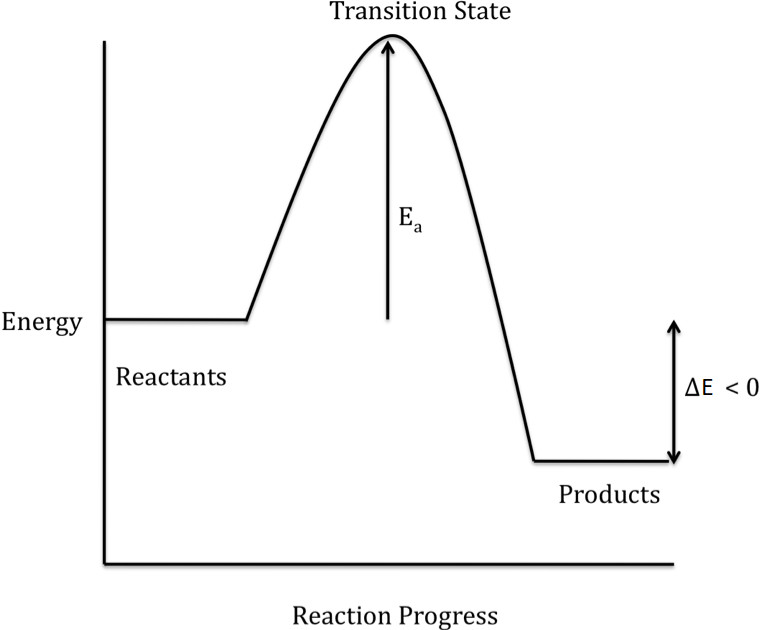
\includegraphics[width=0.35\textwidth]{reactionProfileEsp}
        \caption{Profile reaction.}
    \end{figure}

    \np{Methane is eliminated in a bimolecular reaction with hydroxyl radical formed from a water molecule break by cosmic radiation of space.\cite{web:metano}}

    \nec{CH_4 + \cdot OH \rightarrow CH_3 \cdot + H_2O \label{eq:4}}

    \section*{Materials and methods}

    \np{The modeling of the systems $CH_{4}$, $\cdot OH$, transition state $(TS)$, $CH_{3}\cdot$ and $H_{2}O$ was performed with gaussView separately.}

    \np{The calculations were performed with a laptop with an i7-8750H processor with 8GB of RAM.}

    \np{The transition state is describe in \eqref{eq:5} and represent in figure 4.\n}

    % START FIGURE %
    \begin{figure}[h]
        % Reactive %
        \centering
        \begin{minipage}[b]{0.225\textwidth}
            \centering
          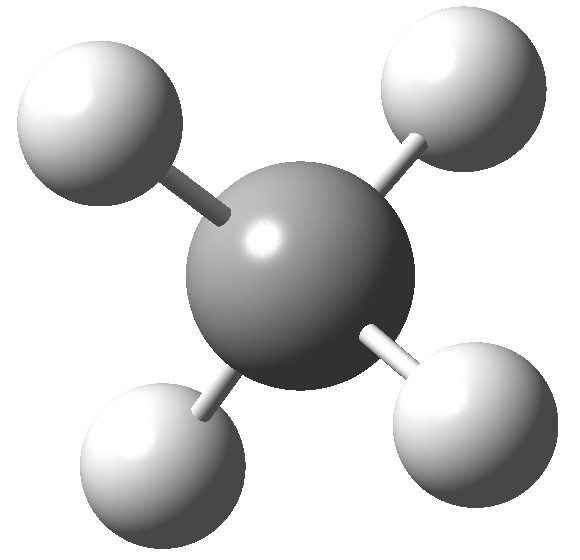
\includegraphics[scale=0.5]{methane}
          \caption{Methane.}
        \end{minipage}
        \hfill
        \begin{minipage}[b]{0.25\textwidth}
          \centering
          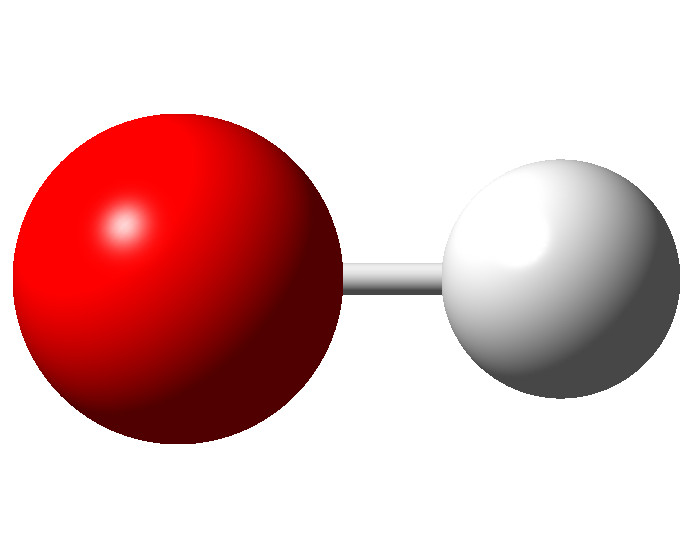
\includegraphics[scale=0.35]{hidroxilRadical}
          \caption{Hydroxyl radical.}
        \end{minipage}
        %Transition state%
        \begin{minipage}[b]{0.45\textwidth}
            \centering
            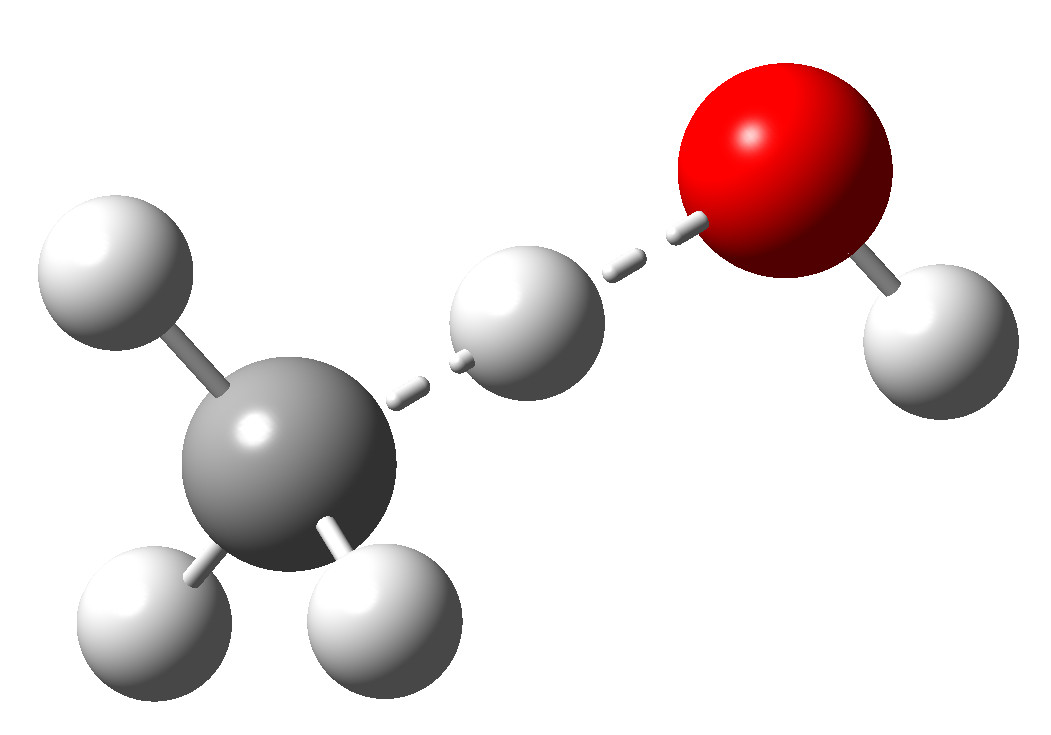
\includegraphics[scale=0.5]{stateTransition}
            \caption{Transition state.}
        \end{minipage}
        %products%
        \centering
        \begin{minipage}[b]{0.225\textwidth}
            \centering
          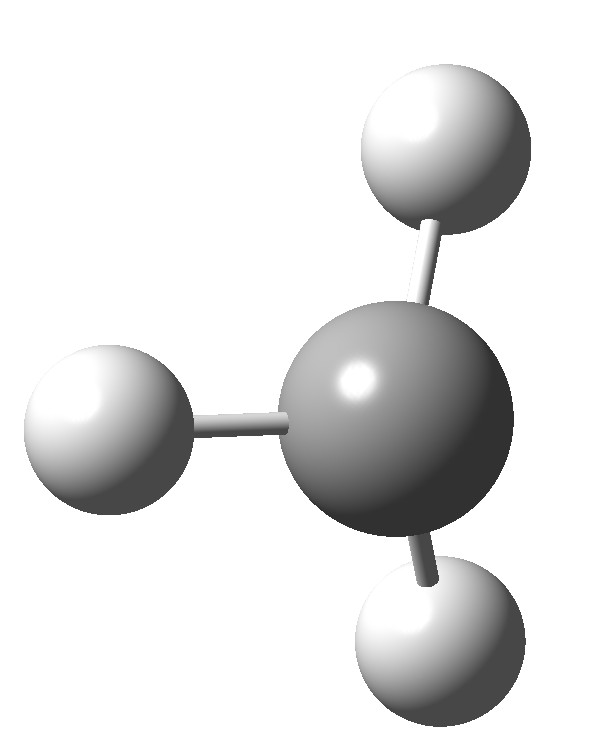
\includegraphics[scale=0.5]{methylRadical}
          \caption{Methyl radical.}
        \end{minipage}
        \hfill
        \begin{minipage}[b]{0.25\textwidth}
          \centering
          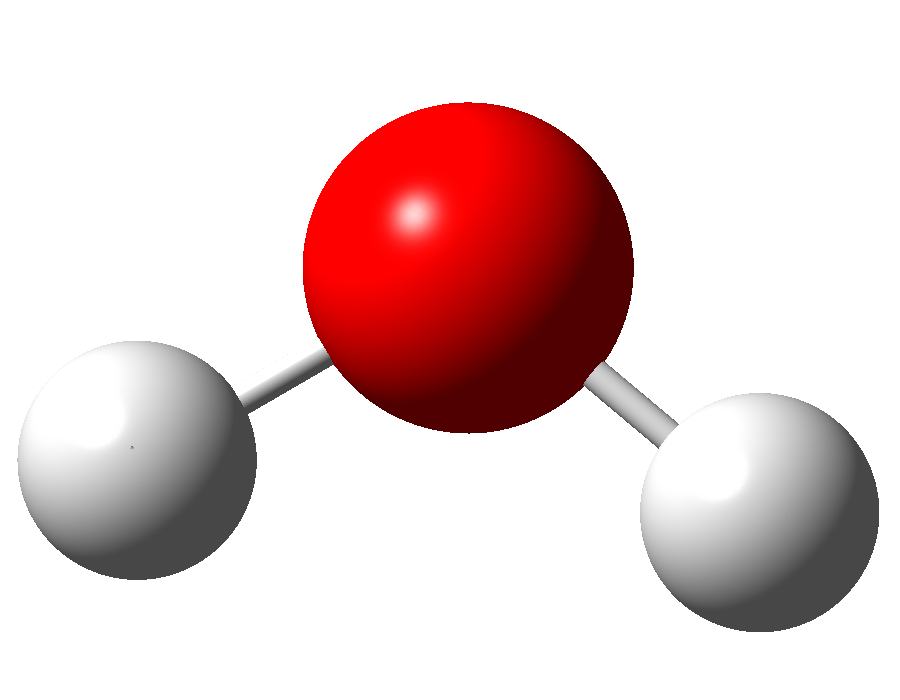
\includegraphics[scale=0.35]{water}
          \caption{Water.}
        \end{minipage}
    \end{figure}
    % END FIGURE %
    \nec{ CH_{4}+\cdot~ OH \rightarrow [ CH_{3}\mbox{-}~\mbox{-}H\mbox{-}~\mbox{-}OH]^{\ddag} \label{eq:5}}

    \np{The input file of reactives and products was running with the following settings. \n}

    \begin{lstlisting}[frame=single,gobble=10] 
            //hardware configuration
            % nprocshared=4
            % mem=1500MB
            //parameters for Method and bases set
            # opt freq X/6-31+G(d) 
    \end{lstlisting}

    \np{X is the methods used HF, B3LYP, and M062X, M062X was run with two bases 6−31+G(d,p) and 6-311++G(d,p) the last was denoted with (*).}
    
    \np{For transition state was calculated with the following settings.\n}

    \begin{lstlisting}[frame=single,gobble=10] 
            //parameters for method
            # opt=(calcfc,ts,noeigen) freq=(noraman)
              x/6-31+g(d,p)
    \end{lstlisting}    
    
    \np{\bt{NOTE:} \em{noeigen} instruction is to tell gaussian to don not stop if find no negative Hessian eigenvalue, \em{ts} and \em{calcfc} calculate the force constants and find vibrations associated with transition state and with ts get the max value of the transition state.}
    
    \section*{Results}
    
    \np{The obtained values were shown in table 1 in the appendix, in table 2 we calculate the values of $\Delta ZPE$, $\Delta H$ and $\Delta G$, in table 3 was show the three points used to build the reaction profile.}

    \titleTable{3}{Reaction profile with $\Delta G$, $\Delta H$, $\Delta ZPE$ in $\frac{kcal}{mol}$.}

    \begin{center} 
        \item \import{./}{table3.tex}
    \end{center}

    \np{With table 3 we build the reaction profile, using each potential, taken as initial reaction coordinate 0.}

    \titleGraph{1}{Free energy VS Reaction coordenate \\ \\}

    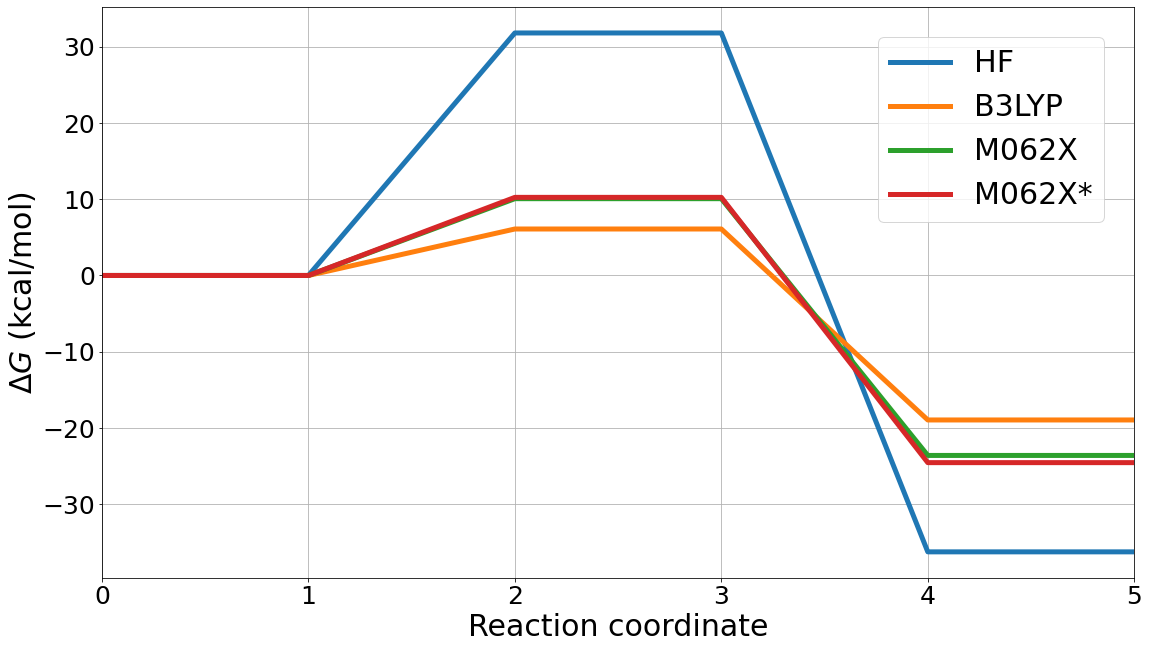
\includegraphics[width=0.49\textwidth]{reactionProfileFreeEnergy}

    \titleGraph{2}{Enthalpy VS Reaction coordenate \\ \\}

    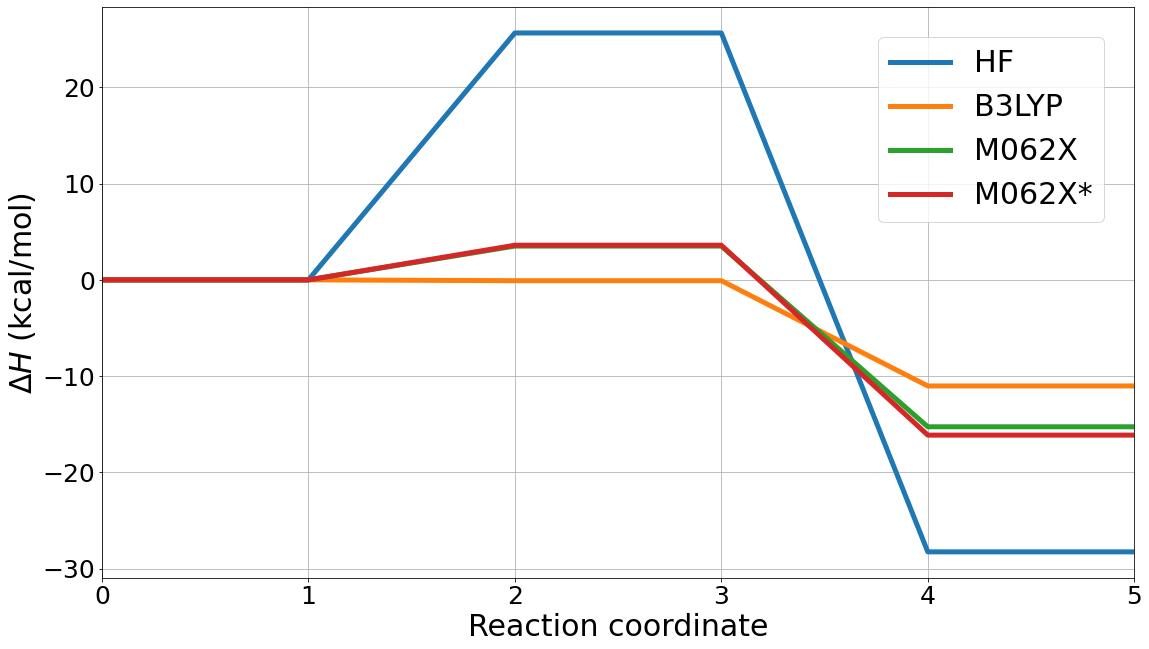
\includegraphics[width=0.49\textwidth]{reactionProfileEnthalpy}

    \titleGraph{3}{ZPE VS Reaction coordenate \\ \\}

    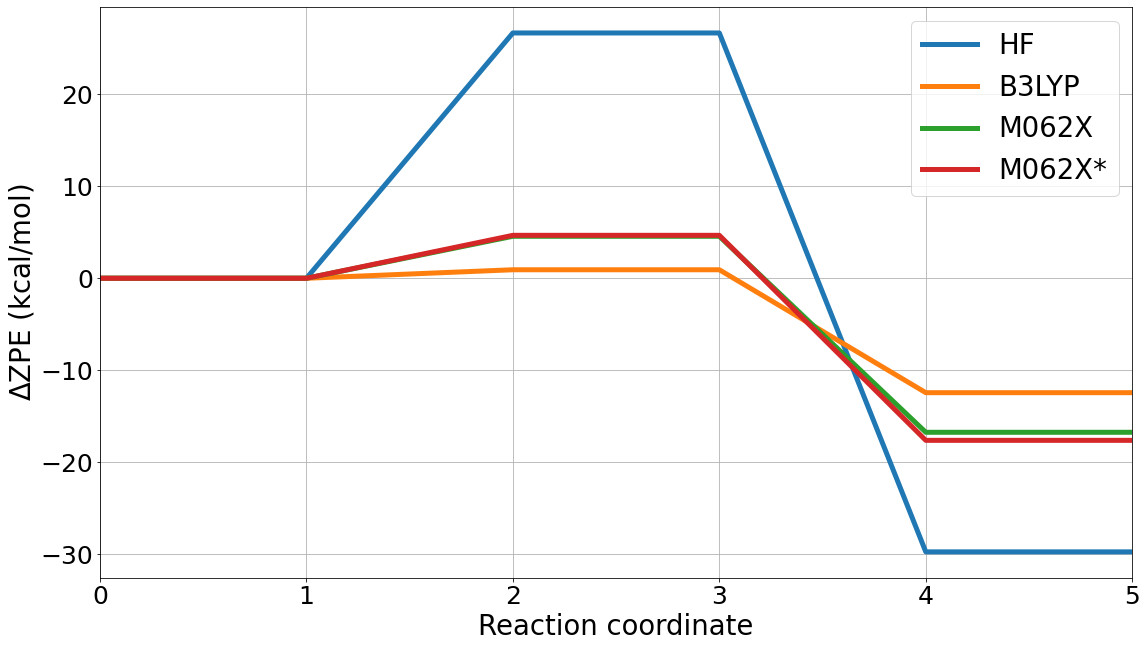
\includegraphics[width=0.49\textwidth]{reactionProfileZPE}

    \np{Using equation \eqref{eq:3} the rate constant were calculated using each method, in this reaction was considered $\kappa=1$ and $\sigma=4$ at 1 atm of pressure, with the experimental value of the rate constant we compared the results $4.07E+06 (s^{-1}M^-1)$ \cite{web:nisg}, and sum the total time of calculation.}

    \titleTable{3}{Rate constant with HF, B3LYP and M062X.}

    \begin{center} 
        \item \import{./}{table4.tex}
    \end{center}

    \section*{Discussion}

    \np{Comparing the reaction profile of $\Delta G$ vs $\Delta H$ showed the fact \textbf{$\Delta G$ and $\Delta H$ cannot be approximated in bimolecular reactions}, the difference of that approximation can be an error like $8 kcal/mol$ like in this case using M062X, in the other hand comparing $\Delta H$ vs $\Delta ZPE$ this approximation is real.}

    \np{Also with graph 1, it shows that reaction is spontaneous, in this case, in particular, \textbf{this reaction has two behaviours is exergonic and exothermic.}}

    \np{With table 4 we can analyze el performance of used methods to calculate the rate constant, first HF does not work this gives us a rate constant 16 orders slower than experimental, B3LYP gives a better approximation but give us 3 orders faster than the real value, in this calculation was corroborated that \textbf{M062x is a method very good to make kinetic} give a rate constant, in this case, was get a value six times faster than original using the basis set 6-31+G.}

    \np{And another point important was the comparison with another basis set, in the graphs, we appreciated a little change of $\Delta G$ or $\Delta H$ for the M062x with different basis set, this gave us a better value with 6-311G++ we get a value only 4 times faster than the experimental value, this tells us the improvement to use a bigger basis set, but consider that the calculus has a bigger cost in computational time of approx 33\%, \textbf{this shows us that the method contributes much more to a good result than using a larger basis set.}}
    %% END SECTION %%
    

    %% START REFERENCES %% 




    % DEFINE STYLE FORMAT%
    \bibliographystyle{ieeetr}
    % SPECIFY THE FILE NAMEw %
    \bibliography{references}

    %START APPENDIX (always in last page)%
    \appendix
    % CHANGE FROM X COLUMN TO ANOTHER COLUMNS EJ 2 -> 1%
    \onecolumn
    \section{Appendix}
    \begin{center}
        \item \titleTable{1}{Values of $G$, $H$, $ZPE$ and Time of running}
        \item \import{./}{anexo1.tex}
    \end{center}

    \begin{center}
        \item \titleTable{2}{Values for profile of reaction of $\Delta G$, $\Delta H$, $\Delta ZPE$}
        \item \import{./}{anexo2.tex}
    \end{center}




    %% END REFERENCES %% 

    %%% THIS CONTENT IS IN TWO COLUMN (END) %%%

\end{document}
%%%%%%%%%%%%%%%% END DOCUMENT %%%%%%%%%%%%%%%%